\documentclass[a4paper, 10pt, twocolumn]{scrartcl}

% Vorlage fuer Poster
% Getestet mit pdfTeX; Kodierung: UTF8
% Version 2024-02-23

% Hier Titel, Name und Modul eintragen:
\newcommand{\thema}{Titel des Posters} % bei mehrzeiligem Thema \posterHeadHeight erhöhen
\newcommand{\name}{Ihr Name}
\newcommand{\modul}{Name des Moduls}

\newcommand{\posterHeadHeight}{29mm}

% Einträge für das Literaturverzeichnis:
\begin{filecontents}[force]{literatur.bib}
@book{knuth,
  author        = {Knuth, Donald E.},
  title         = {The Art of Computer Programming},
  subtitle      = {Fundamental Algorithms},
  volume        = {1},
  publisher     = {Addison-Wesley},
  location      = {Reading, Massachusetts},
  edition       = {3},
  year          = {1997}
}

@online{scheme,
  author        = {Shinn, Alex and Cowan, John and Gleckler, Arthur A.},
  title         = {Scheme Reports Process},
  year          = {2013},
  urldate       = {2020-07-13},
  url           = {http://www.scheme-reports.org/}
}
\end{filecontents}

\usepackage[style=numeric, backend=biber, bibencoding=utf8]{biblatex}
\usepackage{poster}

\begin{document}
% ============================== Block ==============================

\begin{block}{Textauszeichnung}
Text kann unter anderem \emph{kursiv} oder \textbf{fett} gesetzt werden. Lorem ipsum dolor sit amet, consetetur sadipscing elitr, sed diam nonumy eirmod tempor invidunt.
\end{block}

% ============================== Block ==============================

\begin{block}{Abbildungen}
Lorem ipsum dolor sit amet, consetetur sadipscing elitr, sed diam nonumy eirmod tempor invidunt ut labore.

\begin{center}
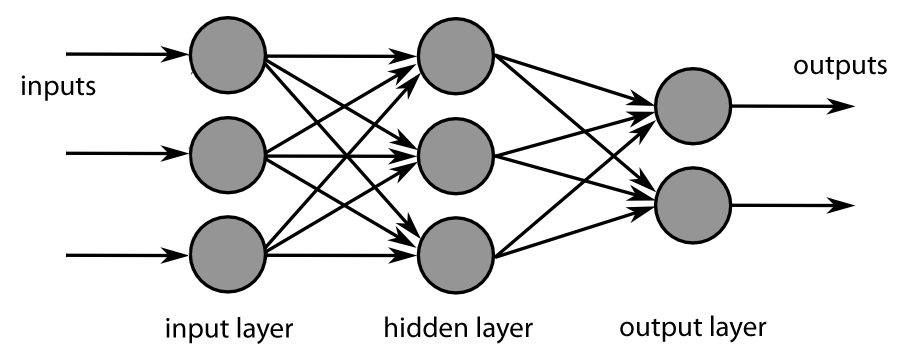
\includegraphics[width=1.0\linewidth]{deeplearning}
\captionof{figure}{Beschreibung der Abbildung.}\label{beispielbild}
\end{center}

Stet clita kasd gubergren, no sea takimata sanctus est Lorem ipsum dolor sit amet. Lorem ipsum dolor sit amet, consetetur sadipscing elitr.
\end{block}

% ============================== Block ==============================

\begin{block}{Zitieren}
Zitat aus \cite{scheme} und \cite[17]{knuth}. Abbildung \ref{beispielbild} und Tabelle \ref{beispieltabelle} können referenziert werden. Lorem ipsum dolor sit amet, consetetur sadipscing elitr, sed diam nonumy eirmod tempor invidunt ut labore et dolore magna aliquyam erat, sed diam voluptua. At vero eos et accusam et justo duo dolores et ea rebum. Lorem ipsum dolor sit amet, consetetur sadipscing elitr, sed diam nonumy eirmod tempor invidunt ut labore et dolore magna aliquyam erat, sed diam voluptua.
\end{block}

% ============================== Block ==============================

\begin{block}{Aufzählungen}
Eine Aufzählung:

\begin{itemize}
\item Lorem ipsum
\item dolor sit amet
\item consetetur sadipscing elitr
\item sed diam nonumy
\end{itemize}

Eine nummerierte Aufzählung:

\begin{enumerate}
\item Erster Punkt
\item Zweiter Punkt
\item Dritter Punkt
\end{enumerate}
\end{block}

% ============================== Block ==============================

\begin{block}{Tabellen}
Eine Tabelle:

\begin{center}
\begin{tabular}{lrc}
\toprule
Linksbündig & Rechtsbündig & Zentriert \\
\midrule
Lorem &  13 & amet \\
ipsum & 104 & consetetur \\
dolor &   7 & sadipscing \\
sit   &  -5 & elitr \\
\bottomrule
\end{tabular}
\captionof{table}{Beschreibung der Tabelle.}\label{beispieltabelle}
\end{center}
\end{block}

% ============================== Block ==============================

\begin{block}{Programmcode}
Code im Fließtext: \lstinline{printf("Hello, world!\n");}. Lorem ipsum dolor sit amet, consetetur sadipscing elitr, sed diam nonumy eirmod tempor invidunt ut labore et dolore magna aliquyam erat, sed diam voluptua. At vero eos et accusam et justo duo dolores et ea rebum.

\begin{lstlisting}
def factorial(x):
    if x <= 1:
        return 1
    return x * factorial(x - 1)
\end{lstlisting}

Stet clita kasd gubergren, no sea takimata sanctus est Lorem ipsum dolor sit amet.
\end{block}

% ----- ab hier nichts mehr ändern -----
\begin{block}{Literatur}
\printbibliography[heading=none]
\end{block}
\end{document}
